\documentclass[english]{article}

%\usepackage[T1]{fontenc}
\usepackage[latin9]{inputenc}
\usepackage[letterpaper]{geometry}
\geometry{verbose,tmargin=1in,bmargin=1in,lmargin=1in,rmargin=1in}
\usepackage{babel}
\usepackage{amsmath}
\usepackage{amssymb}
\usepackage{capt-of}
\usepackage{graphicx}
\usepackage{color}
\usepackage{latexsym}
\usepackage{xspace}
\usepackage{pdflscape}
\usepackage[hyphens]{url}
\usepackage[colorlinks]{hyperref}
\usepackage{enumerate}
\usepackage{ifthen}
\usepackage{float}
\usepackage{array}
\usepackage{tikz}
\usepackage{multirow} 
\usetikzlibrary{shapes}
\usepackage{algorithm2e}
\usepackage{listings}
\usepackage{verbatim}
%%%% HW instructions / collaboration text

\newcommand{\HWPoliciesmix}{
\paragraph*{Instructions.} {\bf This homework contains two parts. Part A is written assignment and Part B is MATLAB programming assignment.}
}

\newcommand{\HWPolicies}{
\paragraph*{Instructions.} 
Please write up your responses to the following problems clearly and
concisely. We encourage you to write up your responses using \LaTeX{};
we have provided a \LaTeX{} template, available on Canvas, to
make this easier. {\bf Submit your answers in PDF form to Canvas. We will not accept paper copies of the homework.}

\paragraph*{Collaboration.} 
You are allowed and encouraged to work together. You may discuss the
homework to understand the problem and reach a solution in groups up
to size {\bf four students.} However, {\em each student must write
  down the solution independently, and without referring to written
  notes from the joint session. {\bf In addition, each student must
    write on the problem set the names of the people with whom you
    collaborated.}} You must understand the solution well enough in
order to reconstruct it by yourself. (This is for your own benefit:
you have to take the exams alone.)
}
\newcommand{\ProgrammingPolicies}[1]{
\paragraph*{Instructions.} 
This is a MATLAB programming assignment. This assignment consists of
multiple parts. Portions of each part will be graded automatically,
and you can submit your code to be automatically checked for
correctness to receive feedback ahead of time.

We are providing you with codebase / templates / dataset that you will
require for this assignment. Download the file {\tt hw#1\_kit.zip}
from Canvas {\bf before} beginning the assignment.  {\bf Please
  read through the documentation provided in ALL Matlab files before
  starting the assignment.} The instructions for submitting your
homeworks and receiving automatic feedback are online on the wiki:

\begin{center}
\url{http://alliance.seas.upenn.edu/~cis520/wiki/index.php?n=Resources.HomeworkSubmission}
\end{center}

\paragraph*{Collaboration.} 
For this programming assignment, you are allowed to work in pairs, but no more than 2. Each group
is required to submit {\bf ONCE} only. {\bf The LOWEST grade will be recorded for multiple submissions.}
Be sure to include your pennkeys and names in the {\it Group.txt} file.
Failure to do so will result in a failure in the grading process. 
{\bf We will be using automatic checking software to detect blatant copying of other student's assignments, so,
please, don't do it.}
}

%%%% CUSTOM COMMANDS FOR FORMATTING EXAMS/HOMEWORKS
\newcounter{section_points}[section]
\newcounter{header_points}[section]
\newcounter{total_points}

\newcommand{\hpoints}[1]{
  \setcounter{header_points}{#1}
  \textbf{[#1 points]}
}

\newcommand{\points}[1]{
  \addtocounter{section_points}{#1}
  \addtocounter{total_points}{#1}
  \textbf{[#1 
    \ifthenelse{\equal{#1}{1}}
    {point}{points}]}
}

\newcommand{\bpoints}[1]{
  \textbf{[#1 
    \ifthenelse{\equal{#1}{1}}
    {point}{points}]}
}


\newcommand{\point}{\textbf{[1 point]}}

\newboolean{ShowSolutions}
\newcommand{\Mistake}[2]{
  \ifthenelse{\boolean{ShowSolutions}}
  {\paragraph{\bf $\blacksquare$ COMMON MISTAKE #1:} {\sf #2} \bigskip}
  {}
}

\newcommand{\Solution}[2]{
  \ifthenelse{\boolean{ShowSolutions}}
    {
      \paragraph{\bf $\bigstar $ SOLUTION:} { \sf
        #1} \bigskip
    }
    { 
      #2
    } %} \vspace{1.5in}}
}
\newcommand{\out}[1]{}

\newboolean{ShowPointsInfo}

\newcommand{\PointStats}[0]{
  \ifthenelse{\boolean{ShowPointsInfo}}
  {
    \begin{center}

      \begin{tabular}{rl}
        \hline
        Stated Points: & \arabic{header_points} \\
        Section Points: & \arabic{section_points} \\
        Total Points So Far: & \arabic{total_points} \\
        \hline 
        \multicolumn{2}{c}{
          
          \ifthenelse{
            \equal{\value{section_points}}{\value{header_points}}
          }{CORRECT TOTAL}
          {{\bf INCORRECT TOTAL}}
          }
          \\
        \hline
      \end{tabular}
    \end{center}
  }{}
}

\newcounter{blankcount}
\newcommand{\myrepeat}[2] {
\setcounter{blankcount}{1}
\whiledo{\value{blankcount} < #1}{
#2
\addtocounter{blankcount}{1}
}
}

\newcommand{\blank}[1]{\underline{\myrepeat{#1}{\qquad}}}


%%%% CUSTOM MATH GOES HERE

\newcommand{\ind}[1]{\mathbf{1}\left(#1\right)}
\renewcommand{\Pr}{\mathbf{Pr}\xspace}
\newcommand{\Bern}{\textsf{Bernoulli}\xspace}
\newcommand{\sign}{\textsf{sign}}

\newcommand{\E}{\mathbf{E}}
\newcommand{\bx}{\mathbf{x}}
\newcommand{\bX}{\mathbf{X}}
\newcommand{\by}{\mathbf{y}}
\newcommand{\bY}{\mathbf{Y}}
\newcommand{\bz}{\mathbf{z}}
\newcommand{\bw}{\mathbf{w}}
\newcommand{\bl}{\mathbf{\ell}}
\newcommand{\vc}[1]{\mathbf{#1}}

\newcommand{\Hypo}{\mathcal{H}}
\newcommand{\XX}{\mathcal{X}}
\newcommand{\cD}{\mathcal{D}}

\newcommand{\argmax}{\operatornamewithlimits{argmax}}
\newcommand{\argmin}{\operatornamewithlimits{argmin}}

\newcolumntype{M}{>{$\vcenter\bgroup\hbox\bgroup}c<{\egroup\egroup$}}

\newcolumntype{x}[1]{>{\centering\arraybackslash}m{#1}}






\title{CIS 520, Machine Learning, Fall 2017: Assignment 6 \\
	Due: Friday, November 10th, 11:59pm \\
	\points{100}}
\date{}
\author{Your Name Here}

\begin{document}
\maketitle

\paragraph*{Instructions.} 
Please write up your responses to the following problems clearly and
concisely. 
We encourage you to write up your responses using \LaTeX{}; we have provided a \LaTeX{} template, available on Canvas, to make this easier. 
{\bf Submit your answers in PDF form to Canvas. 
	We will not accept paper copies of the homework.}

Note, there is no automatic grader for this homework but you do need to submit your code for grading. 
Please add your MATLAB code snippets inline with your solutions. We encourage you to use  \(\mathtt{mcode}\) or \(\mathtt{listings}\) packages for \LaTeX. Code submitted separately will not be graded.

\paragraph*{Collaboration.} 
You are allowed and encouraged to work together. You may discuss the homework to understand the problem and reach a solution in groups up to size {\bf two students.} 
However, each student must write down the solution independently, and without referring to written notes from the joint session. 
{\bf In addition, each student must write on the problem set the names of the people with whom you collaborated.
	It is OK to submit the exact same code used by the partner who you listed in this HW submission.}
You must understand the solution well enough in order to reconstruct it by yourself. (This is for your own benefit: you have to take the exams alone.) \\

{\normalsize \noindent Collaborators: \\
\\ \underline{ Type Collaborator Name Here        }}

\section{CCA\hpoints{13}}

Canonical correlation analysis (CCA) is a method similar to PCA, but
instead of finding the directions of maximum variance (or minimum reconstruction error) within a matrix,
it handles the situation that each data point (i.e., each observation) has two
representations (i.e., two sets of features or ``views''), e.g., a web page can be
represented by the text on that page, and can also be represented by
other pages linked to that page. 

As a simple example, assume each data point has two
representations $x$ and $y$, each of which is a 2-dimensional feature
vector, i.e., $x = [x_1; x_2]^T$ and $y = [y_1; y_2]^T$. Note that in general $x$ and $y$ can have different
numbers of features in them. Given a set of data
points, CCA finds a pair of projection directions $(u; v)$ to maximize the
sample correlation $corr[(u^T x),(v^T y)]$ along the directions $u$ and $v$. In
other words, after we project the $x's$ onto $u$
and the $y's$ onto  $v$, the two projected
representations $u^T x$ and $v^T y$ should be maximally correlated.
Intuitively, data points with large values in one projected direction
should also have large values in the other projected direction.

\begin{enumerate}
\item \points{5} 
Consider the data points shown in the figure below. 
The data $x$ and $y$ are paired -- each point in the left figure corresponds to a specific point in the right figure and vice versa, since these two points are two representations (views) of the same object. 
Different objects are shown in different gray scales in the two figures (so you should be
able to approximately figure out how points are paired). In the right figure we've given one CCA projection
direction $v$, draw the other CCA projection direction $u$ in the left figure. (Problem adapted from Yi Zhang at CMU.)

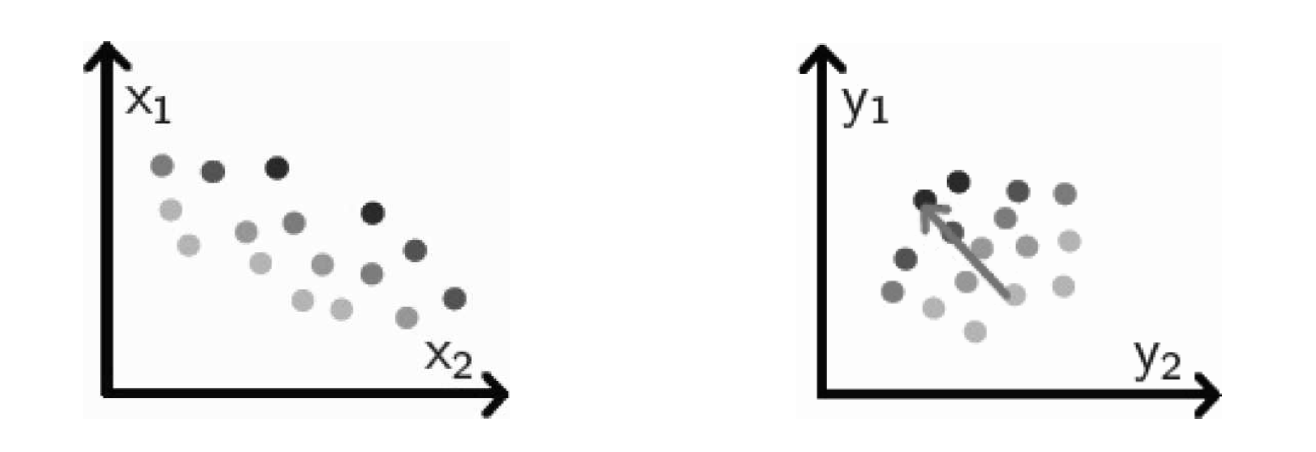
\includegraphics[width=0.6\textwidth]{images/cca.png}


\item \points{8} 
The formal solution for CCA is that the projections $U$ and $V$ are the (largest) left and right singular vectors of
$Z=(X^TX)^{-1/2} X^TY (Y^TY)^{-1/2}$ where $X$ and $Y$ are the two ``views'' of the data, each containing $n$ observations. 
Using the breast cancer data in \(\mathtt{breast\_cancer.mat}\), define \(\mathtt{X=X\_train}\) and \(\mathtt{Y=Y\_train}\) and compute the single largest left and right singular vectors for the matrix \(Z\) as described above.
These are the ``canonical vectors'' .
Here, $X$ is of dimension $n \times p_x$, $Y$ of dimension $n \times p_y$,
$U$ of dimension $p_x \times k$, and $V^T$ of dimension $p_y \times k$.  Since we keep only one (largest) component, $k=1$ in this case.


\begin{enumerate}
\item What is the correlation between  $XU$ and $YV^T$? 
This asks how correlated the two different estimates of the 'hidden state' from the two views are. 
CCA tries to make this number as big as possible.
Note that in this problem  we are looking at the ``degenerate'' case which the $y$ view has only a single feature.

\item How does the above compare to the correlation between $\hat{y}$ and $y$ where 
$\hat{y}$ is this the result of estimating $y$ using only a single principle component, i.e. principle components regression (PCR) with a single component.

%(e.g., as done with $k=1$ on the previous problem.

\end{enumerate}


\end{enumerate}

\section{Sensational EM \hpoints{23}}

Suppose we have a robot with a single unreliable range sensor. For
example, if the robot is standing 3 meters away from the nearest
obstacle, we might get readings like this:
\begin{figure}[h!]
  \centering
  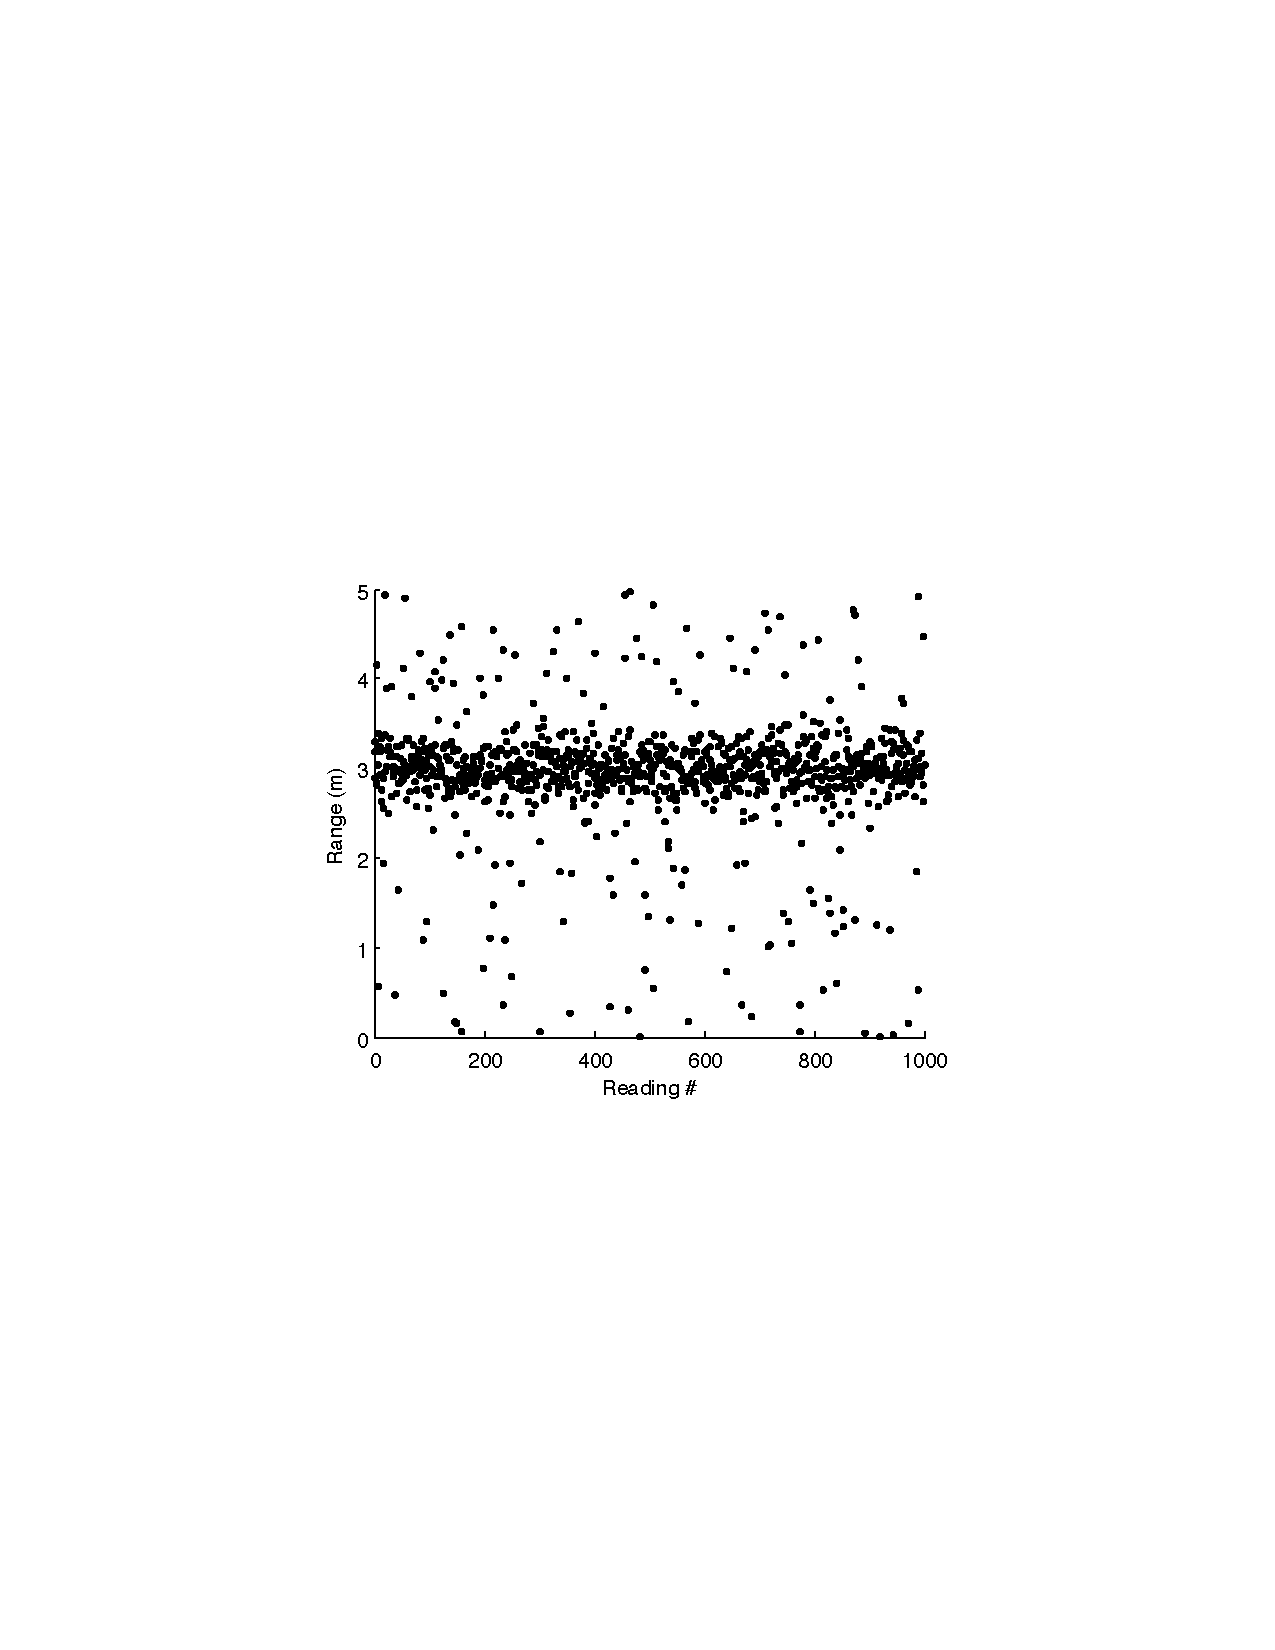
\includegraphics[scale=0.5]{images/range_readings}
  \caption{Range readings from sensor}
  \label{fig:range}
\end{figure}

If the sensor fails when obtaining a reading, it returns a value with
uniform probability in the range $[0,5]$. Otherwise, the sensor
returns a value distributed according to $N(\mu, \sigma^2)$, where
$\sigma^2$ is the variance of the sensor readings and $\mu$ is the
actual distance to the nearest obstacle. We will assume that
$\sigma^2$ is specified by the manufacturer of the sensor, and our
goal is to determine $\mu$ given a set of readings $x_1,\dots,x_n$.

The difficulty is that $\pi_0$, the failure rate of the sensor, is
unknown ahead of time, and we want to avoid biasing our estimate of
$\mu$ with completely meaningless samples where the sensor
failed. Therefore, we model a sensor reading $x_i$ according to the
outcome of a latent variable $z_i$ indicating whether or not the
sensor failed:
\begin{equation*}
  \label{eq:em-model}
  p(z_i = 0) = \pi_0,
  \qquad  p(x_i \mid z_i = 1) = \frac{1}{\sqrt{2\pi}\sigma} \exp \left\{ -\frac{1}{2\sigma^2}(x_i-\mu)^2 \right\},
  \qquad p(x_i \mid z_i = 0) = \frac{1}{5}\mathbf{1}(0\le x_{i}\le5)
\end{equation*}
This is a {\em mixture model} with two components: a Gaussian with
mean $\mu$ and variance $\sigma^2$, and a uniform over $[0,5]$.

%%%%%%%%%%%%%%%%%%%%%%%%%%%%%%%%%%%%%%%%%%%%%%%%%%%%%
\begin{enumerate}
\item \points{4} Using the equations defined above, write out the
  expression for the {\em marginal log likelihood} of a dataset $x_1,
  \dots, x_n$ given the parameters (this is what maximum likelihood is
  maximizing). Your solution should be in terms of $\pi_0, \sigma^2,
  \mu,$ and the $x_i$. {\em Hint: Remember to marginalize over the
    $z_i$'s.}  Write your final answer as: $\log p(x_1,\dots,x_n \mid
  \mu,\sigma^2,\pi_0) = \textrm{expression}$. Please show all your work/derivation for full credits.


%%%%%%%%%%%%%%%%%%%%%%%%%%%%%%%%%%%%%%%%%%%%%%%%%%%%%
\item \points{4} (E-Step) For fixed $\mu,\pi_0$, and $\sigma^2$,
  compute the posterior probabilities $q(z_i = 0 \mid x_i) = p(z_i = 0
  \mid x_, \mu,\pi_0,\sigma^2)$.  Hint: Remember $P(B \mid A) = P(A
  \mid B)P(B)/\sum_B P(A \mid B)P(B)$.  Your solution should be in
  terms of $\pi_0, \sigma^2, \mu,$ and the $x_i$.  Write your final
  answer as: $q(z_i = 0 \mid x_i) = \textrm{expression}$. Please show all your work/derivation for full credits.
  
  
%%%%%%%%%%%%%%%%%%%%%%%%%%%%%%%%%%%%%%%%%%%%%%%%%%%%%
\item \points{5} (M-step for $\mu$) Given the estimates of the
  posterior $q(z_i = 0 \mid x_i)$ and fixed $\pi_0$ and $\sigma^2$,
  now write down the update of $\mu$.  Your solution can include any
  of the following terms: $q(z_i = 0 \mid x_i), \pi_0, \sigma^2$ and
  the $x_i$.  Write your final answer as: $\mu = \textrm{expression}$. Please show all your work/derivation for full credits.


  
%%%%%%%%%%%%%%%%%%%%%%%%%%%%%%%%%%%%%%%%%%%%%%%%%%%%% 
\item \points{5} (M-step for $\pi_0$) Given the estimates of the
  posterior $q(z_i = 0 \mid x_i)$, updated $\mu$, and fixed
  $\sigma^2$, now write down the update for $\pi_0$.  Your solution
  can include any of the following terms: $q(z_i = 0 \mid x_i), \mu,
  \sigma^2$ and the $x_i$.  Write your final answer as: $\pi_0 =
  \textrm{expression}$. Please show all your work/derivation for full credits.
  

    
%%%%%%%%%%%%%%%%%%%%%%%%%%%%%%%%%%%%%%%%%%%%%%%%%%%%%
\item \points{5} Suppose we will now apply our EM procedure to the
  sample dataset in Figure$~\ref{fig:range}$. If we initialize $\mu = 0$ and $\pi_0 = 1/100$
  (with parameter $\sigma^2 = 1/2$) we get the following distribution
  for $q(z_i = 0 \mid x_i)$ as a function of the observation $x_i$:
  \begin{center}
    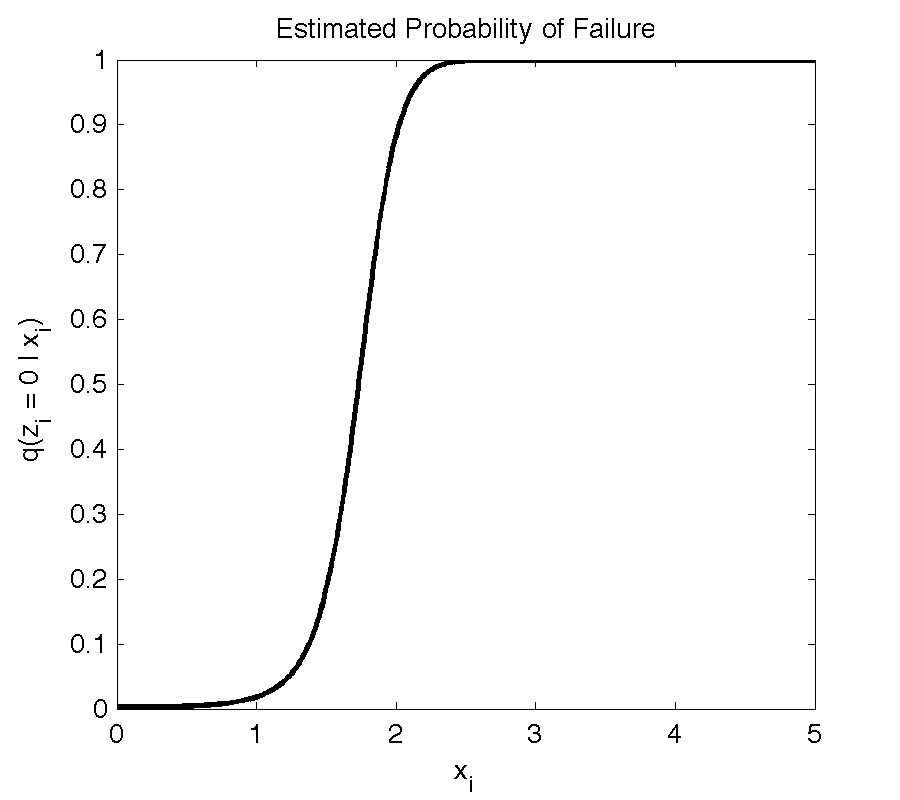
\includegraphics[width=0.4\textwidth]{images/q_mean0.png}
    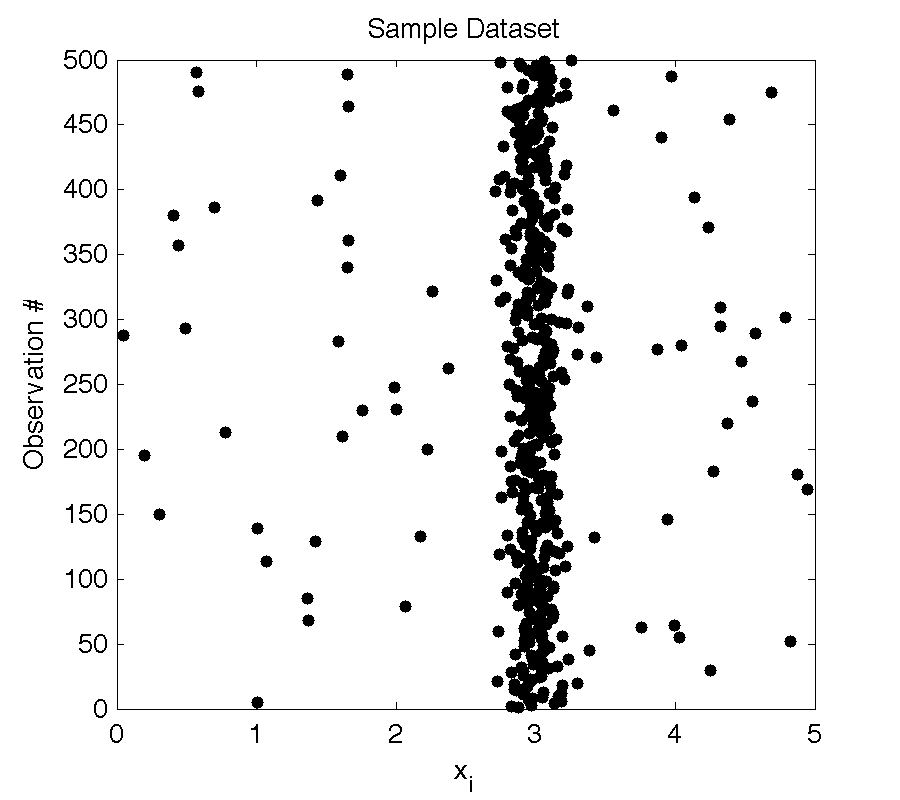
\includegraphics[width=0.4\textwidth]{images/range2.png}
  \end{center}
  Note that the plot of the data has been rotated to align with the
  plot of $q(z_i = 0 \mid x_i)$. 
  
  Will the EM algorithm converge to the correct $\mu$ value given this initialization?
  Briefly explain (2-3 sentences) your answer. Can you provide a better initialization in this situation?
  
  %Briefly explain (2-3 sentences) why we might expect this failure to
  %happen, given the above $q(z_i = 0 \mid x_i)$ distribution. 
  {\em Hint: Look at where the majority of points lie with respect to
    $q(z_i = 0 \mid x_i)$. How will this affect the update for $\pi_0$
    and $\mu$?}


\end{enumerate}

\section{K-Means \hpoints{23}}
%%%%%%%%%%%%%%%%%%%%%%%%%%%%%%%%%%%%%%%%%%%%%%%%%%%%%
Given a set of points $\mathbf{x}_1, \dots, \mathbf{x}_n$, recall that the objective of $K$-means clustering is to minimize within-class sum of squares
\begin{equation*}
  \label{eq:kmeans-model}
	J(\mu,r) = \sum_{i=1}^n\sum_{k=1}^K r_{ik} ||\mu_k-\mathbf{x}_i||^2_2
  \end{equation*}
where $\mu_1,\ldots,\mu_K$ are the centroids of the clusters and $r_{ik}$ are binary variables indicating whether data point $\mathbf{x}_i$ belongs to cluster $k$. 

The optimization is NP-hard. Instead, as described in class, 
the following greedy iterative clustering algorithm is used to alternatively update $\mu_k$ and $r_{ik}$ to optimize $J(\mu,r)$:
\begin{itemize}
 \item Initialize $K$ cluster centroids at random
 \item  Alternate until convergence:
\begin{itemize}
  \item  Assignment step: Assign points to the nearest centroid\\
\begin{equation*}
\arg \min_r J(\mu,r) \rightarrow r_{ik} = \textbf{1}(k = \arg \min_{k'} ||\mu_{k'} - \mathbf{x}_i||_2^2)
 \end{equation*}
 
  \item  Update step: Set the centroid to be the mean of the points assigned to it\\
  \begin{equation*}
 \arg \min_\mu J(\mu,r) \rightarrow \mu_k = \frac{\sum_i r_{ik} \mathbf{x}_i}{\sum_i r_{ik}}
  \end{equation*}
  \end{itemize}
\end{itemize}

%%%%%%%%%%%%%%%%%%%%%%%%%%%%%%%%%%%%%%%%%%%%%%%%%%%%%
\begin{enumerate}
\item \points{3} The greedy iterative clustering algorithm converges when the assignments no longer change. Is the algorithm guaranteed to converge in a finite number of steps? Briefly explain why or why not.\\
{\em Hint: Think about the total possible number of assignments and the trend of the objective function after each iteration.}


%%%%%%%%%%%%%%%%%%%%%%%%%%%%%%%%%%%%%%%%%%%%%%%%%%%%%
\item \points{20} Consider the toy 2D dataset in the following
  Figure~\ref{fig:kmeans_a} and Figure \ref{fig:kmeans_b}. We set $K = 3$ in this problem. The $*$ marker indicates the
  data points and the colored markers (blue circle, green triangle and red square) indicate the 3 starting cluster centroids. 
  Notice that we have a slight different initiation from part $(a)$ to part $(b)$, but it might converge to very different results. 
  For both cases, show the update step and assignment step for each iteration until the algorithm converges. 
  You can use as many of the blank figures (Figure$~\ref{fig:kmeans_blank}$) provided as you need.

Please note that the first update step is given as the
initialization. For each iteration, use one figure to mark the updated
centroids based on the assignment from last iteration, then indicate the data point assignment based on the updated centroid. We expect you to
understand the detailed procedure of $K$-means. You should be able to
compute the centroids manually with a calculator and assign data
points with geometric intuition. Please be sure to show the
coordinates of each centroid in every iteration.

What to hand in? You can
\begin{itemize}
\item \textit{scan:} use your phone or a scanner to take the image with your circle
and include it in the .pdf you hand in, or
\item \textit{write on pdf:} use a pdf tool like adobe acrobat to write directly on the pdf, or
\item \textit{use MATLAB:} run a MATLAB program, and just hand in the outputs at each iteration with the centroids and the list of points in each cluster (but you should see graphically what is happening).
\end{itemize}

\begin{figure}[H]
	\centering
	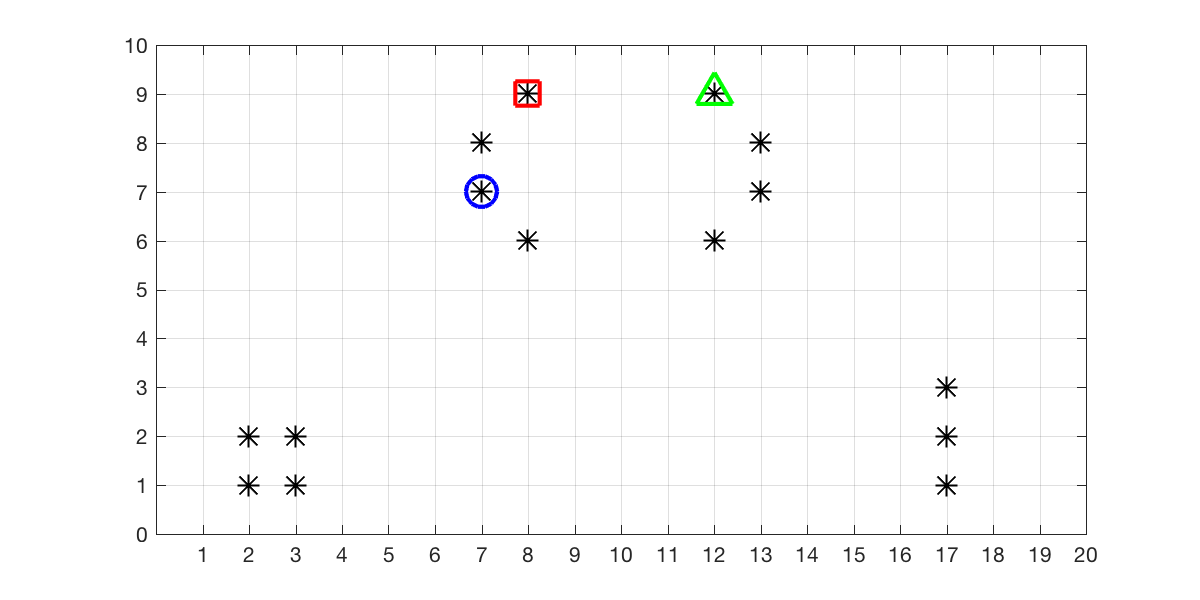
\includegraphics[scale=0.6]{images/k-means_0}
	\caption{Part (a): Dataset with first initialization for K-means.}
	\label{fig:kmeans_a}
\end{figure}

\begin{figure}[H]
	\centering
	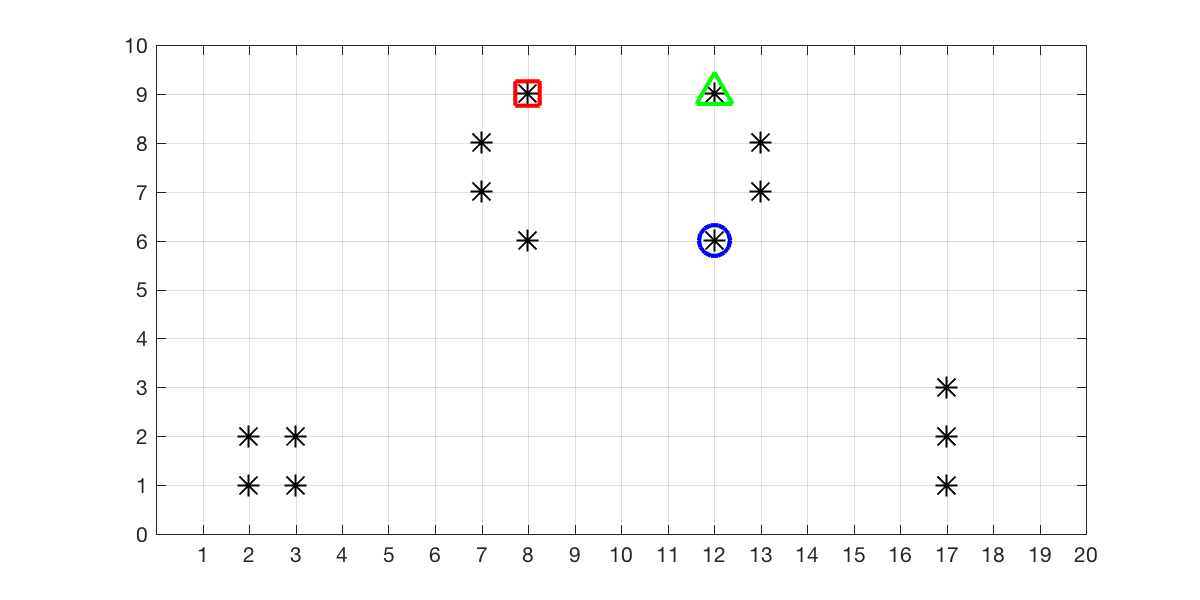
\includegraphics[scale=0.6]{images/k-means_20}
	\caption{Part (b): Dataset with second initialization for K-means.}
	\label{fig:kmeans_b}
\end{figure}

\begin{figure}[H]
  \centering
  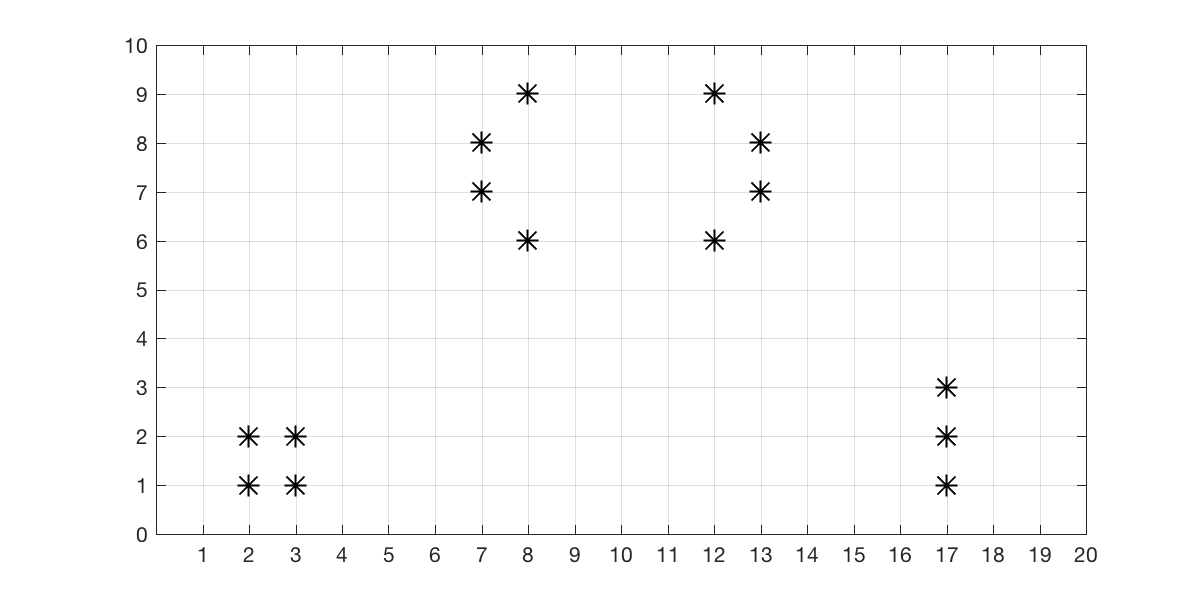
\includegraphics[scale=0.6]{images/k-means_blank}
  \caption{Blank dataset for you to implement K-means.}
  \label{fig:kmeans_blank}
\end{figure}

\end{enumerate}



  

\section{Principal Component Analysis \hpoints{25}}

In this exercise, you will use a part of the MNIST digit dataset, which consists of examples of handwritten digits. Training data is provided in \(\mathtt{MNIST\_train.mat}\) and test data in \(\mathtt{MNIST\_test.mat}\). Each example is a $28 \times 28$ grayscale image, which leads to $784$ pixels to use as features. Each of the labels is shifted by $1$, i.e. the label for the digit '$0$' is $1$ and so on.

You will use PCA to reduce the training data (the pixel data of the training set) from 784 dimensions to 100 dimensions. To 
answer the questions you need to write code in MATLAB to process
the dataset. You {\bf are} allowed to use built-in MATLAB functions for PCA, K-means, fitgmdist, etc. for this problem.

\begin{enumerate}

\item \points{5} Using the top 2 PCA dimensions, display all the test
  digits ``0'' and ``1'', using circles and crosses respectively.
  An example of a plot of ``3'' vs ``4'' is shown in Figure. 1 below. All correct axes, title, and legend must be included.
  Note that the sign of loadings are abitrary (i.e. [-1,1] is the same as [1,-1]).

  \begin{figure}[h!]
    \centering
    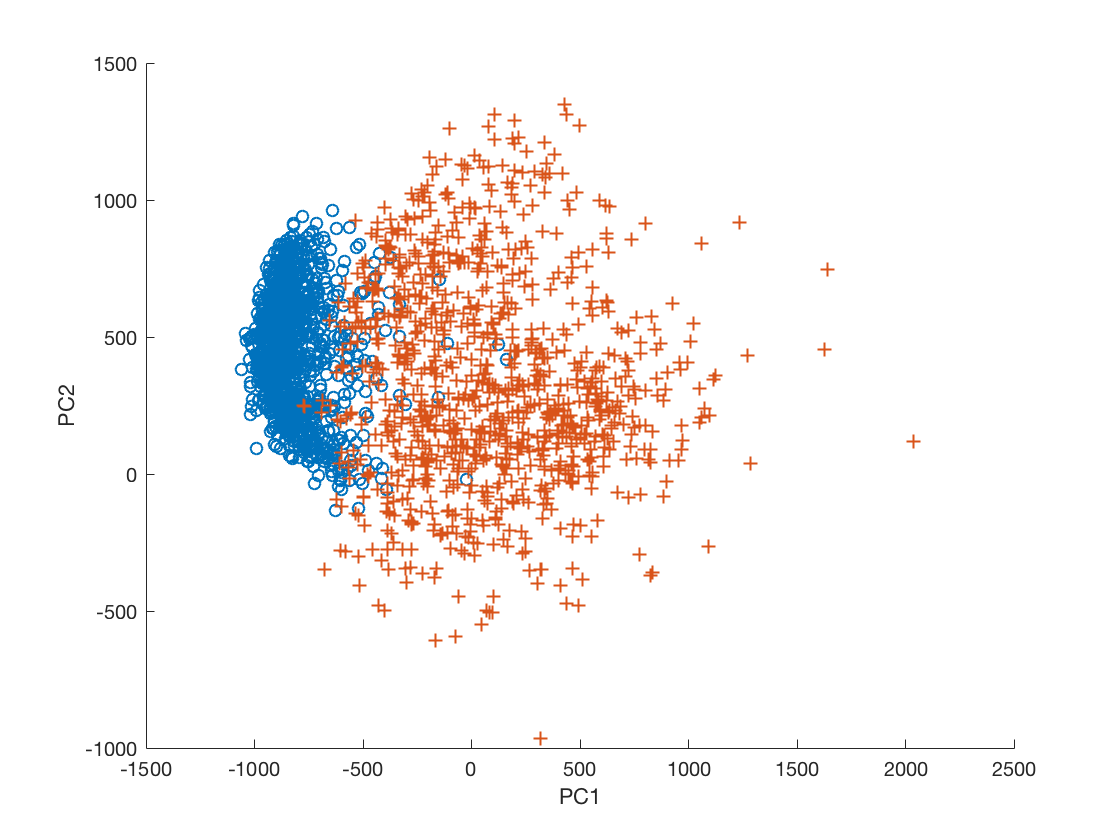
\includegraphics[width=0.65\textwidth]{images/pca_2_vs_3}
    \caption{Plot of '2'-'3' digits from top 2 PCA
        dimensions}\label{fig:pca_2_vs_3}
  \end{figure}
  

\item \points{5} Plot the average (in sample) reconstruction error  $||X - \hat{X}||_F^2$
of the digits as a function of the number of principle components that are included.  How many
principal components are required to get 85\% reconstruction accuracy? (i.e., to explain 85\% of the 
variance: $||\hat{X}-\bar{X}||_F^2/ ||X - \bar{X}||_F^2 = 0.85$ where $\bar{X}$ is a matrix, every row of which is the
average $x$ -- the average image)  
Reminder: make sure you understand the MATLAB function you used, especially whether the function standardize the dataset before running PCA 
and please state it clearly in your solution.


\item \points{10} Cluster the data into 10 clusters using k-means and assign a digit to each cluster.
Report the accuracy on the test set using 100, 150 and 200 top dimensions.
Also state that whether the method you use standardizes the dataset. 

\textbf{Notes:}
  \begin{itemize} 
  \item Please use the following class assignment rule: count the class labels in each cluster, and choose the most popular class (mode) as the label for that cluster.
  \item You can use MATLAB's builtin \(\mathtt{pca}\) and \(\mathtt{kmeans}\) functions. Please read the documentation and understand how to use them.
  \item Both the PCA and the k-means should be trained only on the training set.
  \end{itemize}

\item \points{2} What is the major drawback with the above method, and please name one way to improve it?


\item \points{3} Rerun the above algorithm with 25 clusters using 100, 150, and 200 top dimensions and report the accuracy on the test set. Again, state whether your method standardizes the dataset.

  
\end{enumerate}

\section{Semi-supervised learning \hpoints{16}}

In this exercise, we will use the Optical Character Recognition (OCR) data set (47,000 samples).
See \(\mathtt{ocr\_train.mat}\) which contains \(\mathtt{X\_train}\)  and \(\mathtt{Y\_train}\), and  \(\mathtt{ocr\_test.mat}\) which contains \(\mathtt{X\_test}\)  and \(\mathtt{Y\_test}\).
Specifically, we will examine how a neural network auto-encoder and PCA affect the performance of a model. 
We will compare the performance of logistic regression and k-means using new features obtained from PCA and auto-encoder.

\begin{enumerate}
\item \points{4} \textbf{PCA:}
Use MATLAB function \(\mathtt{pcacov.m}\) on the covariance matrix of  \(\mathtt{X\_train}\) to train coefficients for each principle component. 
See \(\mathtt{pca\_getpc.m}\) for details.
For PCA, choose the number of principle components so as to keep 90\% reconstruction accuracy.
How many principle components do we need in this case? 
Use that many principle components for the rest of analysis. \\

\textbf{Auto-encoders:}
For unsupervised neural nets, which are also known as auto-encoders,
instead of minimizing the error with respect to the ground truth, these models are trained to minimize the input reconstruction error (i.e. treating input as ground truth). 
See \(\mathtt{rbm.m}\) for details of training an auto-encoder. 
Auto-encoders can be viewed as models that learn a new non-linear feature representation. 
That is, we can take the output of a hidden layer of a trained auto-encoder and use it as input features to a supervised learning method. 
We will examine if auto-encoders can learn a good feature representation (by projecting the data set into a higher dimension) and help to improve the performance of a supervised model.


\item \points{6} Now we will perform logistic regression on 3 different inputs:
\begin{itemize}
\item The original features (all 64 dimensions),
\item The PCA-ed data, and 
\item The auto-encoder outputs. 
\end{itemize}

To learn an auto-encoder on the original features, use \(\mathtt{rbm.m}\).
To generate new features from the learned auto-encoder, use \(\mathtt{newFeature\_rbm.m}\).
Write your code in \(\mathtt{test.m}\).

You will do 26-way logistic regression (labels 1, 2, \dots 26) and use an \(L_0\) evaluation of the error (e.g. you get it right or get it wrong).  A useful MATLAB function for this is \(\mathtt{liblinear}\). See \(\mathtt{test.m}\) for an example.
Compare the accuracy on the test set using three different inputs as described above. Compare the accuracy? What's your observation?


\item \points{6} Repeat the steps using K-means, with K = 26, 50 respectively, run the code on original data, PCA-ed data and auto-encoder. Compare the accuracy on the test set, what are the accuracies? Also, compare the performance of K-means with that of logistic regression.

\end{enumerate}


\end{document}
